\section*{Introduction}

\subsection*{Introduction}

\begin{frame}{Le contrôle moteur}
    \begin{block}{But}
        Amener un {\em système mécanique} d'un {\em état} initial à un état désiré
        \begin{center}
            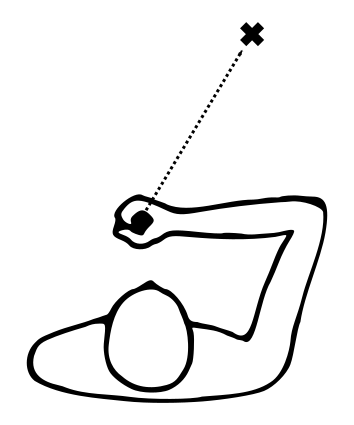
\includegraphics[width=.40\linewidth]{fig/path}
        \end{center}
    \end{block}
\end{frame}

\begin{frame}{La boucle de contrôle}
    \begin{center}
        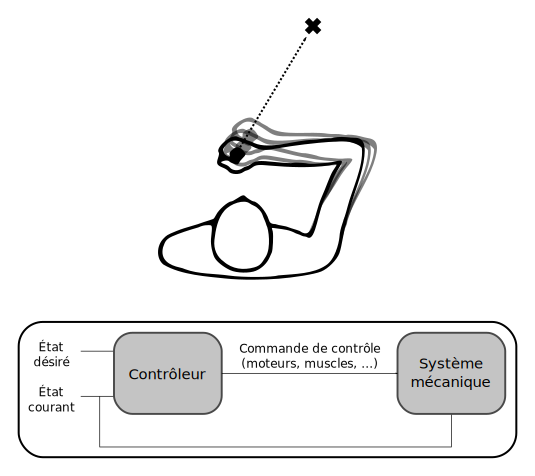
\includegraphics[width=.70\linewidth]{fig/ctrl2}
    \end{center}
\end{frame}

\begin{frame}{Nos objectifs}
    \begin{columns}
        \begin{column}{0.50\textwidth}
            \begin{itemize}
                \item Faire du contrôle moteur sur un système complexe 
                \item Générer des mouvements réalistes et efficaces en reproduisant les propriétés connues du contrôle moteur humain
                %\item Faire un contrôleur pouvant être appris avec les techniques actuelles d'IA
            \end{itemize}
        \end{column}
        \begin{column}{0.50\textwidth}
            \begin{center}
                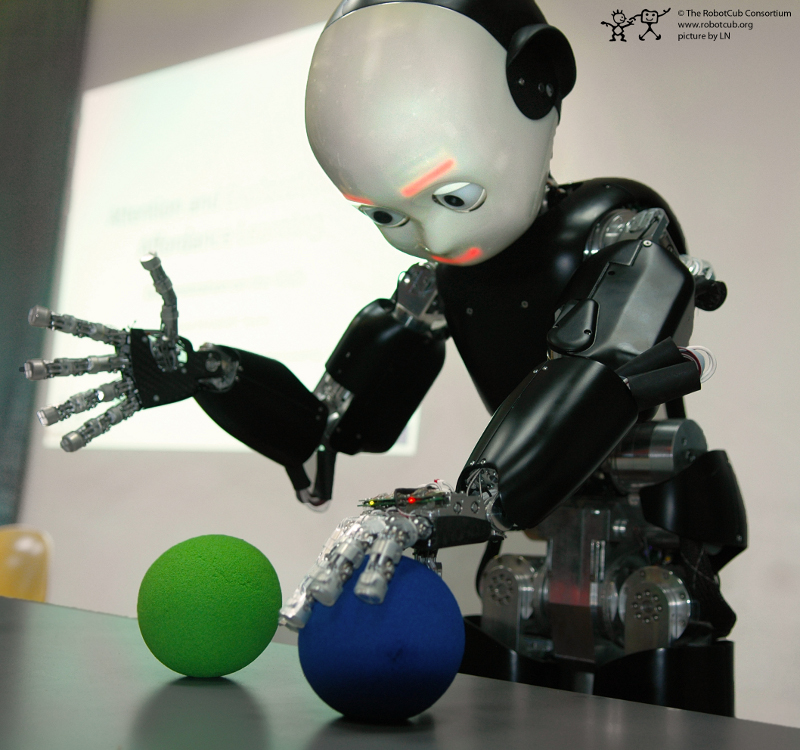
\includegraphics[width=.95\linewidth]{fig/icub_light}
            \end{center}
        \end{column}
    \end{columns}
\end{frame}

\subsection*{Problématique}

\begin{frame}{Problèmes}
    \begin{small}
        Les techniques actuelles ne permettent pas de remplir ces 2 conditions à la fois~:
        ~\\
        \begin{columns}
            \begin{column}{0.70\textwidth}
                \begin{block}{Robotique}
                    Systèmes complexes mais mouvement pas \og{}réaliste\fg{} et peu \og{}efficace\fg{} %pas \og{}human like\fg{} $[$RMRC, Toussaint, ...$]$
                \end{block}
                \begin{block}{Contrôle moteur}
                    Systèmes simples seulement %$[$Rigoux et Guigon, Todorov, ...$]$
                \end{block}
                %\begin{block}{IA - Apprentissage}
                %    Systèmes simples seulement (\og{}malédiction de la dimensionalité\fg{})
                %    %\og{}Malédiction de la dimensionalité\fg{} en apprentissage
                %\end{block}
            \end{column}
            \begin{column}{0.30\textwidth}
                \begin{center}
                    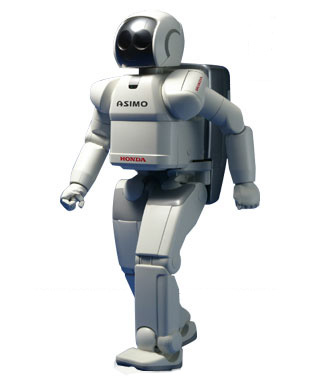
\includegraphics[width=.95\linewidth]{fig/asimo}
                \end{center}
            \end{column}
        \end{columns}
    \end{small}
\end{frame}

%\subsection{Problématique}
%
%%%%%%%%%%%%%%%%%%%%%%%%%%%%%%%%%%%%%%%%
%
%\begin{frame}{Introduction}
%    \begin{figure}
%        \centering
%        \subfigure[Corps humain]{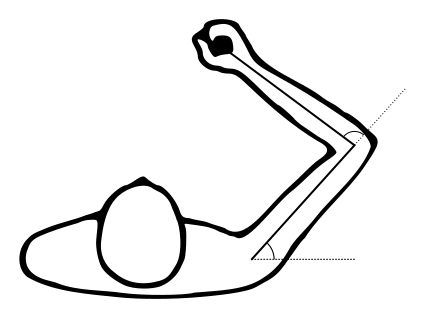
\includegraphics[width=.50\linewidth]{fig/arm4}}~~~
%        \subfigure[Système mécanique poly-articulé]{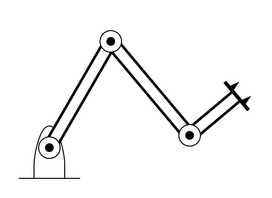
\includegraphics[width=.50\linewidth]{fig/arm1}}
%    \end{figure}
%\end{frame}
%
%\begin{frame}{Introduction}
%    \begin{small}
%        \begin{itemize}
%            \item Système mécanique défini par un état (vitesse position)
%            \item L'état peut être décrit dans plusieurs espaces
%        \end{itemize}
%    \end{small}
%    \begin{figure}[ht]
%        \centering
%        % Note. This illustration was originally made with PSTricks. Conversion to
% PGF/TikZ was straightforward. However, I could probably have made it more
% elegant.

\tikzstyle{blk} = [rectangle, rounded corners, draw=white, very thick, text width=3cm, minimum height=1cm, text centered]

% Define a variable as a length
% Input:
%   #1 Variable name
%   #2 Value
%
% Example:
%   \nvar{\varx}{2cm}
\newcommand{\nvar}[2]{%
    \newlength{#1}
    \setlength{#1}{#2}
}

% Define a few constants for drawing
\nvar{\dg}{0.3cm}
\def\dw{0.25}\def\dh{0.5}
\nvar{\nddx}{0.5cm}

% Define commands for links, joints and such
\def\link{\draw [double distance=1.5mm, very thick] (0,0)--}

\def\joint{%
    \filldraw [fill=white] (0,0) circle (5pt);
    \fill[black] circle (2pt);
}

\def\grip{%
    \node (G) {};
    \draw[ultra thick](0cm,\dg)--(0cm,-\dg);
    \fill (0cm, 0.5\dg)+(0cm,1.5pt) -- +(0.6\dg,0cm) -- +(0pt,-1.5pt);
    \fill (0cm, -0.5\dg)+(0cm,1.5pt) -- +(0.6\dg,0cm) -- +(0pt,-1.5pt);
}

\def\robotbase{%
    \node (B) {};
    \draw[rounded corners=8pt] (-\dw,-\dh)-- (-\dw, 0) --
        (0,\dh)--(\dw,0)--(\dw,-\dh);
    \draw (-0.5,-\dh)-- (0.5,-\dh);
    \fill[pattern=north east lines] (-0.5,-1) rectangle (0.5,-\dh);
}

% Draw an angle annotation
% Input:
%   #1 Angle
%   #2 Label
% Example:
%   \angann{30}{$\theta_1$}
\newcommand{\angann}[2]{%
    \begin{scope}[red]
    \draw [dashed, red] (0,0) -- (1.2\nddx,0pt);
    \draw [->, shorten >=3.5pt] (\nddx,0pt) arc (0:#1:\nddx);
    % Unfortunately automatic node placement on an arc is not supported yet.
    % We therefore have to compute an appropriate coordinate ourselves.
    \node at (#1/2-2:\nddx+8pt) {#2};
    \end{scope}
}

% Define the kinematic parameters of the three link manipulator.
\def\thetaone{60}
\def\Lone{2}
\def\thetatwo{-110}
\def\Ltwo{2}
\def\thetathree{90}
\def\Lthree{1}

\begin{tikzpicture}
    \small

    \robotbase
    \angann{\thetaone}{$q_1$}
    \link(\thetaone:\Lone);
    \joint
    \begin{scope}[shift=(\thetaone:\Lone), rotate=\thetaone]
        \angann{\thetatwo}{$q_2$}
        \link(\thetatwo:\Ltwo);
        \joint
        \begin{scope}[shift=(\thetatwo:\Ltwo), rotate=\thetatwo]
            \angann{\thetathree}{$q_3$}
            %\lineann[0.7]{\thetathree}{\Lthree}{$L_3$}
            \draw [dashed, red,rotate=\thetathree] (0,0) -- (1.2\nddx,0pt);
            \link(\thetathree:\Lthree);
            \joint
            \begin{scope}[shift=(\thetathree:\Lthree), rotate=\thetathree]
                \grip
            \end{scope}
        \end{scope}
    \end{scope}
        
    \node at (1, -1.5) [blk] {Espace articulaire $\q=(q_1~q_2~q_3)^T$};

    \begin{scope}[xshift=5.5cm]
        \robotbase
        \link(\thetaone:\Lone);
        \joint
        \begin{scope}[shift=(\thetaone:\Lone), rotate=\thetaone]
            \link(\thetatwo:\Ltwo);
            \joint
            \begin{scope}[shift=(\thetatwo:\Ltwo), rotate=\thetatwo]
                \draw [dashed, red, rotate=\thetathree] (0,0) -- (1.2\nddx,0pt);
                \link(\thetathree:\Lthree);
                \joint
                \begin{scope}[shift=(\thetathree:\Lthree), rotate=\thetathree]
                    \grip
                \end{scope}
            \end{scope}
        \end{scope}

        \draw [dashed, red] ($(G) + (0mm,  0mm)$) -- ($(G) + (0cm,  -1.6cm)$) node[below] {$x_1$};
        \draw [dashed, red] ($(G) + (0mm,  0mm)$) -- ($(G) + (-4cm,  0cm)$) node[left] {$x_2$};

        % quick & dirty
        %\draw [dashed] ($(B) + (0mm,  -2cm)$) -- ($(G) + (0cm,  -2.5cm)$) node[midway] {$\x$};

        \node at (1, -1.5) [blk] {Espace de la tâche $\x=(x_1~x_2)^T$};
    \end{scope}

\end{tikzpicture}


%    \end{figure}
%    \begin{small}
%    Notations : état  $\jstate = \begin{pmatrix} \dq & \q \end{pmatrix}^T$ et 
%    $\ostate = \begin{pmatrix} \dx & \x \end{pmatrix}^T$
%    \end{small}
%\end{frame}
%
%%\begin{frame}{Problématique}
%%    Redondant dans l'espace de la tâche
%%    \begin{center}
%%        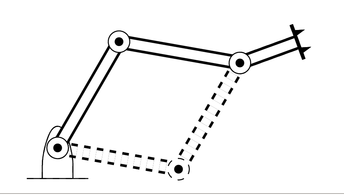
\includegraphics[width=.40\linewidth]{fig/arm2}
%%    \end{center}
%%\end{frame}
%
%\begin{frame}{Problématique}
%    \begin{block}{Une question clé}
%        Pourquoi réalise-t-on tel mouvement plutôt qu'un autre~? $[$Bernstein~67$]$
%    \end{block}
%    \begin{center}
%        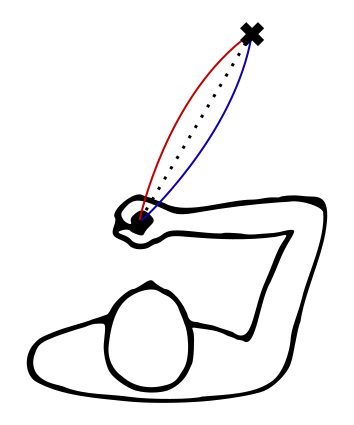
\includegraphics[width=.40\linewidth]{fig/paths}
%    \end{center}
%\end{frame}
%
%%%%%%%%%%%%%%%%%%%%%%%%%%%%%%%%%%%%%%%%
%
%\begin{frame}{Un début de réponse\dots}
%    \begin{block}{Un processus d'optimisation~?}
%        \begin{itemize}
%            \item Pourquoi deux tâches identiques produisent des mouvements différents ?
%            \item Peut-on quantifier ces variations ?
%        \end{itemize}
%    \end{block}
%    Plusieurs propriétés du contrôle moteur ont été identifiées
%    \begin{block}{Principes clés~:}
%        \begin{itemize}
%            \item Minimisation de la variance au point final
%            \item Principe d'intervention minimum
%        \end{itemize}
%    \end{block}
%\end{frame}
%
%%%%%%%%%%%%%%%%%%%%%%%%%%%%%%%%%%%%%%%%
%
%\begin{frame}{Des pistes d'améliorations}
%    Contrôleur de $[$Rigoux et Guigon 11$]$
%    \begin{itemize}
%        \item Reproduit les propriétés du contrôle moteur
%        \item Mais\dots optimise les actions musculaires $\Rightarrow$ trop lent
%    \end{itemize}
%    Regarder le problème sous un autre angle~:
%    \begin{itemize}
%        \item Cinématique
%        \item Dynamique
%        \item Actionnement
%    \end{itemize}
%    Peut-on optimiser sur un plus petit espace ?
%\end{frame}

